\section{API设计}
\label{sec:api-design}

\begin{frame}
  \begin{center}
    \Huge{\textcolor{red}{API设计}}
  \end{center}
\end{frame}

\subsection{mockcpp VS. google mock}

\begin{frame}[fragile]{接口}
  \begin{c++}
class Turtle {
  virtual ~Turtle() {}
  virtual void PenUp() = 0;
  virtual void PenDown() = 0;
  virtual void Forward(int distance) = 0;
  virtual void Turn(int degrees) = 0;
  virtual void GoTo(int x, int y) = 0;
  virtual int GetX() const = 0;
  virtual int GetY() const = 0;  
};
  \end{c++}
\end{frame}

\begin{frame}[fragile]{Google Mock}
  \begin{c++}
#include "gmock/gmock.h"

class MockTurtle : public Turtle {
 public:
  MOCK_METHOD0(PenUp, void());
  MOCK_METHOD0(PenDown, void());
  MOCK_METHOD1(Forward, void(int distance));
  MOCK_METHOD1(Turn, void(int degrees));
  MOCK_METHOD2(GoTo, void(int x, int y));
  MOCK_CONST_METHOD0(GetX, int());
  MOCK_CONST_METHOD0(GetY, int());
};

// Mock Object
MockTurtle turtle;
  \end{c++}
\end{frame}

\begin{frame}[fragile]{mockcpp}
\begin{enumerate}
  \item ABI: Application Binary Interface
  \item 要站在用户的角度定义接口,哪怕背后对应技术实现方式难度更大
  \item 移植性问题(仅支持主流编译器):让90\%的人日子变得好过,总比所有人都难过要好;多数人富起来,少数人贫穷,还是平等,但所有人都平等的贫穷
\end{enumerate}

  \begin{c++}
MockObject<Turtle> turtle;
  \end{c++}
\end{frame}

\subsection{cut VS. google mock}

\begin{frame}[fragile]{Google Test}
\begin{enumerate}
  \item 每个用例都要重复FactorialTest
  \item 遵循严格的标识符命名规则  
\end{enumerate}

  \begin{c++}
TEST(FactorialTest, HandlesZeroInput) {
  EXPECT_EQ(1, Factorial(0));
}

TEST(FactorialTest, HandlesPositiveInput) {
  EXPECT_EQ(1, Factorial(1));
  EXPECT_EQ(2, Factorial(2));
}  
\end{c++}
\end{frame}

\begin{frame}[fragile]{Google Test}
\begin{enumerate}
  \item 为什么要使用protected?
  \item C++98: SetUp/setUp/Setup/setup
\end{enumerate}

  \begin{c++}
class QueueTest : public ::testing::Test {
protected:
  void SetUp() {
    q1_.Enqueue(1);
  }

  Queue<int> q0_;
  Queue<int> q1_;
};
\end{c++}
\end{frame}

\begin{frame}[fragile]{Google Test}
\begin{enumerate}
  \item 区分TEST/TEST\_F
  \item 重复QueueTest
\end{enumerate}

  \begin{c++}
TEST_F(QueueTest, IsEmptyInitially) {
  EXPECT_EQ(0, q0_.size());
}

TEST_F(QueueTest, DequeueWorks) 
{
  q1_.Dequeue();
  EXPECT_EQ(0, q1_.size());
}
\end{c++}
\end{frame}

\begin{frame}[fragile]{CUT: C++ Unified Test Framework}
\begin{enumerate}
  \item 字符串的命名风格
  \item OO风格
  \item ASSERT\_THAT
\end{enumerate}

  \begin{c++}
FIXTURE(QueueTest) {
  Queue<int> q0_, q1_;

  SETUP() {
    q1_.Enqueue(1);
  }

  TEST("is empty initially") {
    ASSERT_THAT(q0_.size(), eq(0));
  }

  TEST("dequeue should works") {
    q1_.Dequeue();
    ASSERT_THAT(q0_.size(), eq(0));
  }
};
\end{c++}
\end{frame}

\begin{frame}[fragile]{Hamcrest: 可扩展性}
  \begin{figure}
    \centering
    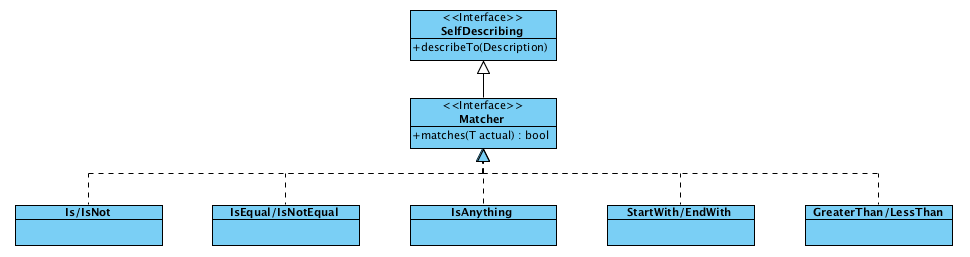
\includegraphics[width=1.0\textwidth]{hamcrest.png}
  \end{figure}
\end{frame}

